\documentclass[letterpaper,10pt]{article}
\usepackage{graphicx}
\usepackage{listings}
\usepackage{fullpage}
\usepackage{fixltx2e}
\usepackage{multirow}
\usepackage{amssymb,amsmath}
\usepackage{mathtools}
\usepackage[hyperfootnotes=false,hidelinks]{hyperref}
\usepackage{url}
\usepackage{subfig}
\usepackage{relsize}
\usepackage{enumitem}
\usepackage{booktabs}
\usepackage{sectsty}
\usepackage{pgffor}
\usepackage{tikz}
\usepackage{cite}
%\usepackage{natbib}
%\sectionfont{\fontsize{14}{16}\selectfont}
%\usepackage{empheq}
%\usepackage[x11names]{xcolor}
%\numberwithin{figure}{section}
%\numberwithin{table}{section}
%\numberwithin{equation}{section}
\usepackage{fancyhdr}
%\setlength{\headheight}{14pt}
\pagestyle{fancy}
%\headsep = 24pt
\linespread{1.0}
%\setlength{\parskip}{0.85\baselineskip}
%\setlength{\parindent}{0pt}

\renewcommand{\arraystretch}{1.2}
\usepackage{xcolor}
\lstset{basicstyle=\ttfamily,
  showstringspaces=false,
  commentstyle=\color{red},
  keywordstyle=\color{blue}
}

% Custom hyphenation
\hyphenation{tur-bu-lence}
\hyphenation{Rey-nolds}


%%%%%%% CODES

\newcommand{\code}{\textit{PyFlowCL}}
\newcommand{\NGA}{\textit{NGA}}
\newcommand{\PlasComCM}{\textit{PlasComCM}}
\newcommand{\PlasComCMtwo}{\textit{PlasCom2}}
\newcommand{\goldenCopy}{\textit{golden copy}}
\newcommand{\GoldenCopy}{\textit{Golden Copy}}
\newcommand{\cl}[1]{\textit{codelet-#1}}
\newcommand{\Cl}[1]{\textit{Codelet-#1}}
\newcommand{\plusplus}[1]{#1{}\texttt{++}}


\newcommand{\Q}[1]{{\medskip\small\noindent\color{red}#1\par}}

%%%%%%% ANIMATIONS
\newcommand{\insertmovie}[3]{\ifmovies{
\movie[autostart,loop]
{\includegraphics[width=#1\textwidth]{Movies/#2}}
{Movies/#3}
}
\else{
\includegraphics[width=#1\textwidth]{Movies/#2}
}
\fi
}


%%%%%%%%% COLORS
%\definecolor{myBlue}{RGB}{19,41,75}  %%% ILLINOIS BLUE
\definecolor{myBlueLink}{RGB}{70,70,200}  %%% ILLINOIS BLUE
\definecolor{myBlue}{RGB}{18,28,43}  %%% ND BLUE
\definecolor{myOrange}{RGB}{26,82,126} % monochromatic lighter
%\definecolor{myOrange}{RGB}{232,74,39}  % IL orange
\definecolor{IllinoisOrange}{RGB}{232,74,39}  %%% ILLINOIS ORANGE
\definecolor{IllinoisBlue}{RGB}{19,41,75}   %%% ILLINOIS BLUE
\definecolor{mainText}{RGB}{18,28,43}  %%% ND BLUE
%\definecolor{mainText}{RGB}{19,41,75}  %%% ILLINOIS BLUE

\definecolor{ForestGreen}{rgb}{0.0, 0.2, 0.13}
\definecolor{darkpastelgreen}{rgb}{0.01, 0.75, 0.24}
\definecolor{antiquewhite}{rgb}{0.98, 0.92, 0.84}

\newcommand{\makeRed}[1]{{\color{red} #1}}


%%%%%%%%% COMMENTS/INSTRUCTIONS/NOTES
\newcommand{\instr}[1]{{\color{red}\footnotesize #1}}
\newenvironment{notes}{\color{red}\footnotesize \begin{center}\begin{minipage}{0.8\textwidth}}{\end{minipage}\end{center}}
\newcommand{\CHK}{{\color{red}CHK???}}
\newcommand{\CHKCS}{{\color{Green}CHK CS ???}}


%%%%%%%%% FORMATTING
\captionsetup{labelfont={color=myOrange,bf},textfont={color=myBlue}}
\newcommand{\HRule}[2]{{\color{myOrange}\rule{#1}{#2}}}
\newcommand{\tPI}[1]{{\color{myOrange}#1}}
\newcommand{\ttPI}[1]{\texttt{\color{myOrange}#1}}
\newcommand{\sPI}[1]{\textsc{\color{myOrange}#1}}
\newcommand{\cPI}[1]{\textbf{\color{myOrange}#1}}
\newcommand{\rPI}[1]{\textrm{\color{myOrange}#1}}
\newcommand{\iPI}[1]{\textit{\color{myOrange}#1}}
\newcommand{\lead}[1]{\textit{\color{myOrange}(#1)}}
\newcommand{\tabtit}[1]{\textsc{\color{myOrange}#1}}
\newcommand{\entry}[1]{\mbox{\sffamily\bfseries{#1:}}\hfil}%
\newcommand{\bitem}{\item[{\color{myOrange}$\bullet$}]}
\newcommand{\oitem}{\item[{\color{myOrange}$\circ$}]}
\newcommand{\cditem}{\item[{\color{myOrange}$\cdot$}]}
\newcommand{\bmath}{\boldsymbol}
\newcommand{\eps}{\varepsilon}
\newcommand{\Dpartial}[2]{\frac{\partial #1}{\partial #2}}
\newcommand{\itemcolor}[1]{% Update list item colour
\renewcommand{\makelabel}[1]{\color{#1}\hfil ##1}}
\newcommand{\cM}{\mathcal{M}}
\newcommand{\gdotfill}{{\color{gray}\dotfill}}
\newcommand{\bvec}[1]{\ensuremath{\boldsymbol{#1}}}
\newcommand{\matrd}[1]{\ensuremath{\mathsf{#1}}}
\newcommand{\cs}[1]{\textcolor{IllinoisOrange}{\texttt{#1}}}
%\newcommand{\parab}[2]{\vspace{#1 pt}\noindent \paragraph{\bf #2 \\}}




\def \d {\mathrm{d}}
\def \dd#1#2{\frac{\mathrm{d} #1}{\mathrm{d} #2}}
\def \pp#1#2{\frac{\partial #1}{\partial #2}}
\newcommand{\dprime}[1]{^{\prime\prime #1}}
\newcommand{\sprime}[1]{^{\prime #1}}
\newcommand{\ol}[1]{\overline{#1}}
\newcommand{\wt}[1]{\widetilde{#1}}
\newcommand{\oll}[1]{\overline{#1}_\lambda}
\newcommand{\wtl}[1]{\widetilde{#1}_\lambda}
\newcommand{\wh}[1]{\widehat{#1}}
\newcommand{\avg}[1]{\left\{ {#1} \right\}}
\newcommand{\avgunw}[1]{\left\langle {#1} \right\rangle}
\newcommand{\bx}{\mathbf{x}}
\newcommand{\bu}{\mathbf{u}}
\newcommand{\bg}{\mathbf{g}}
\newcommand{\bbf}{\mathbf{f}}
\newcommand{\bh}{\mathbf{h}}

\def \avgrho {\avgunw{\rho}}
\newcommand{\olu}{\overline{u}}
\newcommand{\olbu}{\overline{\mathbf{u}}}
\newcommand{\olxi}{\overline{\xi}}
\newcommand{\olrho}{\overline{\rho}}

\newcommand{\wtu}{\widetilde{u}}
\newcommand{\wtbu}{\widetilde{\mathbf{u}}}

\newcommand{\DNSsub}{{\text{\textsc{dns}}}}
\newcommand{\LESsub}{{\text{\textsc{les}}}}
\newcommand{\SGSsub}{{\text{\textsc{sgs}}}}

\newcommand{\la}{\left \langle}
\newcommand{\ra}{\right\rangle}

\newcommand{\cb}[1]{{\color{blue} #1}}
\newcommand{\norm}[1]{\left\lVert #1 \right\rVert}

\def \Da {\mathrm{Da}}
\def \Dad {\mathrm{Da}_\Delta}
\def \Ka {\mathrm{Ka}}
\def \Kaf {\mathrm{Ka}_{\avg{C}=0.5}}
\def \Kacr {\mathrm{Ka}_\mathrm{cr}}
\def \Rey {\mathrm{Re}}
\def \Ma {\mathrm{Ma}}
\def \Pr {\mathrm{Pr}}
\def \Sc {\mathrm{Sc}}
\def \HtwoO {{\mathrm{H}_2\mathrm{O}}}

\newcommand{\bbC}{\mathbb{C}}
\newcommand{\vbbm}{{\vec{m}}}
\newcommand{\bbM}{\mathbb{M}}
\newcommand{\bbH}{\mathbb{H}}
\newcommand{\bbG}{\mathbb{G}}
\newcommand{\bbV}{\mathbb{V}}

\newcommand{\vD}{{\vec D}}
\newcommand{\vhD}{{\hat{D}}}
\newcommand{\vg}{{\vec g}}
\newcommand{\vphi}{{\vec\phi}}
\newcommand{\vtheta}{{\vec\theta}}
\newcommand{\vOmega}{{\vec\Omega}}

\newcommand{\vF}{{\vec{F}}}
\newcommand{\vf}{{\vec{f}}}
\newcommand{\vb}{{\vec{b}}}
\newcommand{\vq}{{\vec{q}}}
\newcommand{\vqs}{{\vec{q}^{\,\color{red}*}}}

\newcommand{\cJ}{\mathcal{J}}
\newcommand{\cG}{\mathcal{G}}
\newcommand{\cI}{\mathcal{I}}
\newcommand{\cP}{\mathcal{P}}
\newcommand{\cN}{\mathcal{N}}
\newcommand{\cC}{\mathcal{C}}
\newcommand{\cO}{\mathcal{O}}

\newcommand{\rstar}{{\color{red}*}}
\newcommand{\rchk}{{\color{red} \checkmark}}
\newcommand{\gchk}{{\color{green} \checkmark}}
\newcommand{\rbul}{{\color{red} $\bullet$}}
\newcommand{\pbul}{{\color{myOrange} $\bullet$}}
\newcommand{\ro}{{\color{red} $\circ$}}

\newcommand{\rhoi}[1][i]{\rho_{#1}}
\newcommand{\dt}[1][t]{\partial_{#1}}
\newcommand{\dx}[1][{\textrm{\bf x}}]{\boldsymbol \partial_{#1}}
\newcommand{\Vi}[1][i]{\mathcal{V}_{#1}}
\newcommand{\Mi}[1][\textswab{i}]{\mathcal{M}_{#1}}
\newcommand{\omegai}[1][i]{\dot{\omega}_{#1}}
\newcommand{\grav}{{\bf g}}
\newcommand{\Etot}{\mathcal{E}}

\newcommand{\mBG}{m_{\text{\tiny BG}}}
\newcommand{\nBG}{n_{\text{\tiny BG}}}
\newcommand{\nIp}{n_{\text{\tiny $I^+$}}}
\newcommand{\nIm}{n_{\text{\tiny $I^-$}}}


\newcommand{\bE}{{\mathbf{E}}}
\newcommand{\bI}{{\mathbf{I}}}
\newcommand{\bq}{{\mathbf{q}}}
\newcommand{\bQ}{{\mathbf{Q}}}
\newcommand{\bF}{{\mathbf{F}}}
\newcommand{\olbq}{{\overline{\mathbf{q}}}}
\newcommand{\btau}{{\boldsymbol{\tau}}}

\newcommand{\bv}{{\bar{v}}}
\newcommand{\bepsilon}{{\bar{\epsilon}}}

\newcommand{\ST}{{S_{\text{\tiny T}}}}

\newcommand{\vu}{\vec{u}}
\newcommand{\vQ}{\vec{Q}}
\newcommand{\veta}{\vec{\eta}}

\newcommand{\TODO}[1]{{\color{pink} \tiny TODO: #1}}
\newcommand{\mynote}[1]{{\color{green} \tiny #1}}
\newcommand{\prj}[2]{{\color{gray} #1 [#2]}}

\newcommand{\myoul}[1]{\color{myOrange}\underline{\smash{\color{pdcolor1} #1}}\color{pdcolor1}}
\newcommand{\ccdot}{\color{myOrange}$\circ$\color{pdcolor1}\;}
\newcommand{\cc}[1]{\color{myOrange}#1\color{pdcolor1}{}}


% Grad, div, curl, etc.
\newcommand{\vdot}{\mathop{\mbox{\boldmath{$\cdot$}}}}
\newcommand{\vddot}{\mathop{\mbox{\textbf{:}}}}
\newcommand{\bnabla}{\mbox{\boldmath{$\nabla$}}}
\newcommand{\Lapl}{\nabla^2}
\newcommand{\hLapl}{\nabla^2_{\!\mathrm{h}}}
\newcommand{\pLapl}{\nabla^2_{\!\!\!\perp}}


% Custom line colors for Gnuplot EPS+LaTeX terminal
\definecolor{lc1}{HTML}{CE282A}
\definecolor{lc2}{HTML}{255BCB}
\definecolor{lc3}{HTML}{009647} %2DCE65}
\definecolor{lc4}{HTML}{A21D8E}
\definecolor{lc5}{HTML}{F1AB65}
\definecolor{lc6}{HTML}{89B6D4}
\definecolor{lc7}{HTML}{A0A0A0}





%%%%%%%%% PAGE DIMENSIONS
\setlength{\oddsidemargin}{0.0in}
\setlength{\textwidth}{6.5in}
\setlength{\topmargin}{-0.3in}
\setlength{\footskip}{0.15in}
\setlength{\textheight}{9.0in}
\setlength{\headheight}{0.2in}
\setlength{\headsep}{0.1in}

%%%%%%%%%%% FLOAT MANAGEMENT
 \renewcommand{\topfraction}{0.9}
    \renewcommand{\bottomfraction}{0.8}
    \setcounter{topnumber}{2}
    \setcounter{bottomnumber}{2}
    \setcounter{totalnumber}{4}     % 2 may work better
    \setcounter{dbltopnumber}{2}    % for 2-column pages
    \renewcommand{\dbltopfraction}{0.9}	% fit big float above 2-col. text
    \renewcommand{\textfraction}{0.07}	% allow minimal text w. figs
    \renewcommand{\floatpagefraction}{0.7}	% require fuller float pages
    \renewcommand{\dblfloatpagefraction}{0.7}	% require fuller float pages

%%%%%%%%%% PARAGRAPHING
\setlength{\parindent}{0pt}
\setlength{\parskip}{1.2ex}
\renewcommand{\baselinestretch}{0.95}


%%%%%%%%% SECTIONING STUFF
\makeatletter
\renewcommand{\section}{\@startsection
{section}%
{0}%
{0mm}%
{1\baselineskip}%
{0.4\baselineskip}%
{%\rule{\linewidth}{0.8pt}\\
  \normalfont\Large\bfseries\color{myOrange}}}%
\makeatother

\makeatletter
\renewcommand{\subsection}{\@startsection
{subsection}%
{1}%
{0mm}%
{1\baselineskip}%
{0.4\baselineskip}%
%{0.01\baselineskip}%
{\normalfont\large\bfseries\color{myOrange}}}%
\makeatother

\makeatletter
\renewcommand{\subsubsection}{\@startsection
{subsubsection}%
{1}%
{0mm}%
{-0.5\baselineskip}%
{0.3\baselineskip}%
%{-0.3\baselineskip}% removes newline
{\normalfont\normalsize\itshape\centering\color{myOrange}}}%
%{\normalfont\normalsize\itshape\color{myOrange}}}%
\makeatother


\renewcommand{\thesection}{\arabic{section}}
\renewcommand{\thesubsection}{\thesection.\arabic{subsection}}


\newcommand{\myhref}[2]{\href{#1}{{\color{myBlueLink} #2}}}

\newenvironment{noinditemize}
{\begin{itemize}[leftmargin=*,label=\color{myOrange}$\bullet$,itemsep=0in]\raggedright}
{\end{itemize}}

\newenvironment{tnoinditemize}
{\begin{tiny}\begin{noinditemize}}
{\end{noinditemize}\end{tiny}}


\newcommand{\jfm}[1]{{\color{magenta}JFM: #1}}



\fancyhf{}
\fancyhead[L]{\code\ Numerics}
\fancyhead[R]{\today}
\fancyfoot[C]{\thepage}

\title{\code\ Numerics}
\author{J.~F.~MacArt and MacRTL Group \\
  Aerospace \& Mechanical Engineering \\
  University of Notre Dame}

\begin{document}

% Title page
\maketitle

\vspace*{10em}
\begin{center}
  \includegraphics[width=7cm]{Figures/cylinder_Mach1.png}
\end{center}

\clearpage

\thispagestyle{plain}
\tableofcontents

\clearpage

\thispagestyle{plain}
\begin{abstract}
\code\ is a 3D, structured, compressible Navier--Stokes solver using curvilinear grids. It discretizes the equations using high-order finite-difference schemes~\cite{Lele1992} and shock-capturing schemes~\cite{Cook2004,Fiorina2007,Kawai2008a}, which make it suitable for both low-speed turbulent flows and high-speed shock-dominated flows. It is Python-native and leverages the \emph{PyTorch} library~\cite{PyTorch} for high-performance machine and GPU offloading. 
\end{abstract}
\vspace{1em}



\section{Governing Equations}

\code\ solves the 3D compressible Navier--Stokes equations in conservative form,
\begin{equation}
  \pp{\bQ}{t} + \pp{\bF_c}{\bx} = \pp{\bF_v}{\bx} + \sigma (\bQ_\mathrm{ref} - \bQ),
  \label{e:NS}
\end{equation}
where $t\geq 0$, $\bx=(x,y)$, $\bQ=(\rho,\rho u,\rho v,\rho E)$, $\rho$ is the density, $\bu=(u,v)$ is the velocity vector, $E=e+\bu^\top\bu/2$ is the total energy, and $e$ is the internal energy. In \eqref{e:NS}, $\bF_c$ are the convective fluxes, $\bF_v$ are the viscous/diffusive fluxes, and $\sigma$ is an absorbing boundary condition (described below) that drives the solution toward a reference state $\bQ_\mathrm{ref}$ where it is active.

%\jfm{Cite Colonius 2004 Annual Rev on boundary conditions?}

The governing equations \eqref{e:NS} are nondimensionalized using a reference length scale $L$ and freestream velocity $u_\infty$, density $\rho_\infty$, pressure $p_\infty$ and temperature $T_\infty$:
\begin{align*}
  \hat t&=\frac{t u_\infty}{L}, &
  \hat\bx&=\frac{\bx}{L}, &
  \hat\rho &= \frac{\rho}{\rho_\infty}, &
  \hat\bu &= \frac{\bu}{u_\infty}, &
  \hat p &= \frac{p}{\gamma p_\infty}, &
  \hat T &= \frac{T}{(\gamma-1)T_\infty}, &
  \hat e &= \frac{e}{u_\infty^2},
\end{align*}
where the ratio of specific heats $\gamma=c_p/c_v$ is taken to be $\gamma=1.4$ for calorically perfect air. This yields the nondimensional governing equations,
\begin{align}
  \pp{\hat\rho}{\hat t} + \pp{\hat\rho\hat u_j}{\hat x_j} &= 0, \label{e:mass} \\
  \pp{\hat\rho\hat u_i}{\hat t} + \pp{\hat\rho\hat u_i\hat u_j}{\hat x_j} + \frac{1}{\Ma^2}\pp{\hat p}{\hat x_i} - \frac{1}{\Rey}\pp{\hat\tau_{ij}}{\hat x_j} &= 0, \label{e:mom} \\
  \pp{\hat\rho\hat E}{\hat t} + \pp{\hat\rho\hat u_j\hat E}{\hat x_j} + \frac{1}{\Ma^2}\pp{\hat p u_j}{\hat x_j} - \frac{1}{\Rey}\pp{\hat u_i\hat\tau_{ij}}{\hat x_j} + \frac{1}{\Ma^2\Rey\Pr}\pp{\hat q_j}{\hat x_j} &= 0, \label{e:energy}
\end{align}
where $i,j=(1,2,3)$, the viscous stress tensor and the heat-flux vector are
\begin{align*}
  \hat\tau_{ij} &= \hat\mu\left[\left(\pp{\hat u_i}{\hat x_j} + \pp{\hat u_j}{\hat x_i}\right) - \frac{2}{3}\pp{\hat u_k}{\hat x_k}\delta_{ij}\right] + \hat\mu_B\pp{\hat u_k}{\hat x_k}\delta_{ij}, \\
  \hat q_j &= -\hat\mu\pp{\hat T}{\hat x_j},
\end{align*}
and a power-law dependence is assumed for the viscosity: $\hat\mu = \mu/\mu_\infty = \left[(\gamma-1)\hat T\right]^{0.7}$.
In \eqref{e:mom} and \eqref{e:energy}, the scaling Mach, Reynolds, and Prandtl numbers are
\begin{align*}
  \Ma &= \frac{u_\infty}{\sqrt{\gamma p_\infty/\rho_\infty}}, &
  \Rey &= \frac{\rho_\infty u_\infty L}{\mu_\infty}, & &\mathrm{and} &
  \Pr &= \frac{c_p\mu_\infty}{\lambda_\infty}.
\end{align*}
The system is closed by the nondimensional ideal gas law: $\hat p = (\gamma-1)\hat\rho\hat T/\gamma$. Noting that $\hat T=\gamma\Ma^2\hat e$ for a calorically perfect gas ($e=c_v T$), the pressure is evaluated using $\hat p=(\gamma-1)\Ma^2\hat\rho\hat e$, with $\hat e$ obtained from the total energy.


%\subsection{Initial Conditions}

%\code\ implements a Grid module (\texttt{Grid.py}) with a separate class for each grid type (enumerated in Sec.~\ref{s:grids}). In addition to generating the grid and coordinate transforms, the Grid classes are also required to implement a member function \texttt{Grid.<className>.get\_IC(Q,U0,gamma,Ma)} that returns the tensor of initial conditions $\bQ_0$. An individual grid class's IC generator can be made capable of initializing multiple ICs by passing additional arguments to the class constructor.



\subsection{Boundary Conditions}

\code\ supports the following types of boundary conditions:
\begin{itemize}
\item Periodic boundaries
\item Isothermal/adiabatic no-slip walls (``wall'')
\item Absorbing layers (``farfield'')
\end{itemize}
Boundary conditions are applied on the computational grid: this means that they will conform to curvilinear boundaries in the physical space. Grid classes are \emph{required} to implement the following boundary condition specifiers:
\begin{itemize}
\item \cs{self.periodic\_xi = \{True,False\}} (if false, farfield boundaries are applied)
\item \cs{self.BC\_eta\_top = \{periodic,wall,farfield\}}
\item \cs{self.BC\_eta\_bot = \{periodic,wall,farfield\}}
\item \cs{self.periodic\_eta = \{True,False\}} (can be set automatically from the preceding options)
\end{itemize}


\subsubsection{Periodic Boundary Conditions}
Periodic boundary conditions can be specified separately in the $\xi$- and $\eta$-directions. Periodic boundary conditions are \emph{required} in the $z$-direction. When enabled, they are applied to all conserved quantities. All derivatives maintain their interior order-of-accuracy at periodic boundaries.


\subsubsection{Wall Boundary Conditions}
Wall boundary conditions apply homogeneous Dirichlet conditions to the velocity components. Neither Dirichlet nor Neumann conditions are appropriate at walls for the density and total (internal) energy. Two types of energy boundary conditions are available at walls:
\begin{enumerate}
\item Isothermal walls ($T=\mathrm{const}$), and
\item Adiabatic walls ($\partial T/\partial n=0$, where $n$ is the surface-normal vector).
\end{enumerate}
Adiabatic walls are physically more realistic for problems with significant wall heating, e.g., aerodynamic flight vehicles at supersonic Mach numbers.


\subsubsection{Absorbing Layers}
Absorbing layers are typically applied to external boundaries $\delta^e\Omega$ at which it is desirable to ensure that pressure waves do not reflect back into the computational domain. A source term controls the local application of the absorbing layers,
\begin{equation}
  \sigma(x,y) = \left\{ \begin{array}{c l}
    \alpha\left(1 - \frac{d((x,y),\partial^e\Omega)}{\delta_\alpha}\right)^p, & d((x,y),\partial^e\Omega)<\delta_\alpha, \\
    0 & \mathrm{otherwise},
  \end{array} \right.
\end{equation}
where $d((x,y),\delta^e\Omega)$ is the distance from a point $(x,y)$ to the boundary $\delta^e\Omega$, $\delta_\alpha$ is the absorbing layer thickness, $\alpha$ is the source-term strength, and $p$ is its polynomial order. These parameters are problem-dependent. A good set of parameters to begin with is $\alpha=5$ and $p=3$. To implement the absorbing layer, source terms $\sigma_k (\bQ_\mathrm{ref}-\bQ)$ are added to the RHS of the governing equation \eqref{e:NS}, where $\bQ_\mathrm{ref}$ is the reference (target) state, and $k\in[0,4]$ specifies one particular boundary. Dirichlet conditions $\bQ=\bQ_\mathrm{ref}$ are then applied on $\partial^e\Omega$.

\code\ supports separate absorbing layers at the top, bottom, left, and right domain boundaries. The source terms $\sigma_k$ are initialized in the Grid module in one of two ways:
\begin{enumerate}
\item Individual grid classes may optionally implement a member function \cs{self.get\_absorbing\_layer} (see the \cs{Grid.cylinder} class for an example). If it exists, then \code\ will use it to set up the source terms. This is the preferred approach for curved farfield boundaries.
\item If the chosen grid class does not implement the member function (1.), then \code\ will use the module function \cs{Grid.get\_absorbing\_layer()} to configure the source terms using the Cartesian ($x$-$y$) distance from the boundaries of the physical-space grid. Because this is based on the Cartesian distance, it is not ideal when applying farfield conditions to curved boundaries.
\end{enumerate}
After obtaining the initial condition, \code\ saves the initial conditions at the boundaries as the target states for any active farfield boundaries.




\section{Numerical Methods}


\subsection{The Computational Grid}

\code\ solves the Navier--Stokes equations \eqref{e:NS} in a general, curvilinear physical space domain $x_i=(x,y,z)$ using coordinate transformations. All derivatives are discretized on a uniform, rectilinear computational grid $\xi_i=(\xi,\eta,z)$, which enables application of arbitrarily high-order finite-difference schemes to irregular physical domains. The computational grid is most often defined in terms of the physical-space domain: $\xi=\xi(x,y)$ and $\eta=\eta(x,y)$.
For example, in an O-type curvilinear grid, $\eta$ represents the radial distance, and $\xi$ represents the polar angle (see Fig.~\ref{fig:curvilinear}).
\begin{figure}
  \centering
  \includegraphics[width=0.75\textwidth]{Figures/curvilinear.pdf}
  \caption{Illustration of an O-type physical-space grid $(x,y)$ and the corresponding computational grid $(\xi,\eta)$. (This document uses $\eta$ in place of $\zeta$ in this figure.)}
  \label{fig:curvilinear}
\end{figure}

For computational efficiency, the $z$-direction is currently strictly uniform and rectilinear. Thus it does not depend on the curvilinear transforms or vice versa. 


\subsection{Computation of Derivatives} \label{sec:transforms}

This section describes the computation of metrics (derivatives) in the physical-space domain under the curvilinear coordinate transform. All discrete derivatives will be taken on the computational grid, so we desire to expand the physical-space derivatives in terms of the computational-space coordinates. To obtain the expressions for the derivatives $\partial/\partial\xi$ and $\partial/\partial\eta$, consider the expansion of the partial derivatives with respect to $x=x(\xi,\eta)$ and $y=y(\xi,\eta)$:
\begin{align*}
  \pp{}{x} &= \xi_x\pp{}{\xi} + \eta_x\pp{}{\eta} \\
  \pp{}{y} &= \xi_y\pp{}{\xi} + \eta_y\pp{}{\eta},
\end{align*}
where we denote $\xi_x=\partial\xi/\partial x$ and so on. It will often be easier to specify $x=x(\xi,\eta)$, $y=y(\xi,\eta)$ than $\xi=\xi(x,y)$, $\eta=\eta(x,y)$, so we seek to replace $\xi_x$ with $x_\xi$, etc. One can show that
\begin{equation}
  \left[ \begin{array}{cc} \xi_x & \xi_y \\
      \eta_x & \eta_y \end{array} \right] =
  \frac{1}{|J|}  \left[ \begin{array}{cc} y_\eta & -x_\eta \\
      -y_\xi & x_\xi \end{array} \right],
  \label{e:inv_transform}
\end{equation}
where $|J|\equiv |\partial(x,y)/\partial(\xi,\eta)| = x_\xi y_\eta - x_\eta y_\xi$ is the determinant of the grid Jacobian matrix. 

Individual Grid classes are required to compute the nodal grid transforms $\xi_x$, $\xi_y$, $\eta_x$, and $\eta_y$ as well as the determinant of the grid Jacobian matrix. Since it is often more convenient to specify $x=x(\xi,\eta)$ and $y=y(\xi,\eta)$ (i.e., to construct the physical-space grid from the computational grid) than to specify $\xi$ and $\eta$ in terms of $x$ and $y$, \code\ uses the inverse transform \eqref{e:inv_transform} and the grid Jacobian to obtain the necessary transforms.

Nodal grid transforms may be obtained in one of two ways:
\begin{enumerate}
\item If the physical-space grid is a simple function of $\xi$ and $\eta$, then the partial derivatives $\partial(x,y)/\partial(\xi,\eta)$ may be obtained analytically. Many Grid classes implement a member function \cs{self.get\_transform(xi,eta)} to compute the necessary partial derivatives (see \cs{Grid.py} for examples).
\item If the physical-space grid is not a simple function of $\xi$ and $\eta$, or if it is specified pointwise, then the Grid module function \cs{Grid.grid\_transform\_2CD()} may be used to compute the partial derivatives and the grid Jacobian. Currently, this is done using second-order central differences; this can contribute larger truncation error than the spatial derivatives for fine meshes. This effect is explored in Section~\ref{sec:verification}. Therefore, this option should be used with caution. (Or change it to use fourth-order derivatives!)
\end{enumerate}




\subsection{Discretization Schemes} \label{s:disc_schemes}

\code\ semi-discretizes the governing equations in the computational plane ($\xi,\eta$) using \textbf{5-point, 4th-order central-difference schemes} and 4th-order boundary schemes (Sec.~\ref{s:disc_schemes}).  An extension to 5-point, 6th-order compact schemes~\cite{Lele1992} is planned. The shock-capturing artificial-diffusivity scheme is based on 4th-order central-difference approximations to the 4th derivative and a truncated Gaussian filter (Sec.~\ref{s:shock_capturing}). Time is advanced using the 4th-order Runge--Kutta method.

Currently, only fourth-order explicit schemes are used for spatial derivatives. The sixth-order compact schemes could be implemented without increasing the stencil width, but the requirement for a tridiagonal solve could negatively affect adjoint-based optimization performance.

\begin{itemize}
  \setlength{\itemsep}{1em}
\item \textbf{First derivatives} are obtained using fourth-order central differences. These are computed from a generalized, seven-point central-difference stencil~\cite{Lele1992}
  \begin{equation}
    %\begin{split}
    \beta f'_{i-2} + \alpha f'_{i-1} + f'_i + \alpha f'_{i+1} + \beta f'_{i+1} = %\\
    a\frac{f_{i+1}-f_{i-1}}{2h} + b\frac{f_{i+2}-f_{i-2}}{4h} + c\frac{f_{i+3}-f_{i-3}}{6h},
    \label{e:firstderiv}
    %\end{split}
  \end{equation}
  where $h$ is the uniform directional grid spacing ($\Delta\xi$, $\Delta\eta$, or $\Delta z$). A one-parameter family of five-point, maximally tridiagonal stencils is obtained from \eqref{e:firstderiv} by setting $\beta=0$ and $c=0$:
  \begin{equation*}
    \beta=0, \qquad a=\frac{2}{3}(\alpha+2), \qquad b=\frac{1}{3}(4\alpha-1), \qquad c=0.
  \end{equation*}
  \begin{itemize}
  \item {Fourth-order explicit:} $\alpha=0$, $a=\frac{4}{3}$, $b=-\frac{1}{3}$, $c=0$
  \item {Sixth-order compact tridiagonal:} $\alpha=\frac{1}{3}$, $a=\frac{14}{9}$, $b=\frac{1}{9}$, $c=0$
  \end{itemize}
  \code\ currently uses the \textbf{fourth-order explicit scheme} with lower-order central and one-sided schemes near wall and farfield boundaries. For example:
  \begin{itemize}
  \item $i=0$ (wall boundary): 2-point, 1st-order one-sided differences,
  \item $i=1$: 3-point, 2nd-order central differences,
  \item $i\geq 2$ (interior): 5-point, 4th-order explicit central.
  \end{itemize}


\item \textbf{Second derivatives} are obtained by repeated application of first derivatives.


\item \textbf{Fourth derivatives} are needed for the artificial-diffusivity scheme.  A generalized seven-point central-difference stencil for the fourth derivative is~\cite{Lele1992}
\begin{equation}
  \alpha f^{iv}_{i-1} + f^{iv}_{i} + \alpha f^{iv}_{i+1} = a\frac{f_{i+2} - 4f_{i+1} + 6f_i - 4f_{i-1} + f_{i-2}}{h^4} + b\frac{f_{i+3} - 9f_{i+1} + 16f_i - 9f_{i-1} + f_{i-3}}{6h^4},
  \label{e:fourthderiv}
\end{equation}
where $h$ is the uniform directional grid spacing. A one-parameter family of seven-point, maximally tridiagonal stencils is obtained from \eqref{e:fourthderiv}.
\begin{itemize}
\item {Fourth-order explicit:} $\alpha=0$, $a=2$, $b=-1$
\item {Sixth-order compact tridiagonal:} $\alpha=\frac{7}{26}$, $a=\frac{19}{13}$, $b=\frac{1}{13}$
\end{itemize}
\code\ currently uses the fourth-order explicit scheme together with lower-order and one-sided boundary schemes.

\end{itemize}

\textbf{Implementation:} Derivatives are implemented in the Metrics module (\cs{Metrics.py}). The module is organized as follows:
\begin{itemize}
\item Metrics class: \cs{class central\_4th\_periodicRectZ()}. Contains:
  \begin{itemize}
  \item \cs{self.grad\_node(q)}: computes $\partial q/\partial (x,y,z)$ required for RHS evaluation. This function has several options:
    \begin{itemize}
    \item The $\partial x$, $\partial y$, and $\partial z$ derivatives can be disabled separately (defaults to enabled).
    \item (Homogeneous) Neumann boundary conditions can be enforced (defaults to false).
    \item Options for computing derivatives on the extended interior or true interior (defaults to true inteiror).
    \end{itemize}
  \item \cs{self.grad4\_node(q)}: computes $\partial^4 q/\partial (\xi,\eta,z)^4$ required for artificial-diffusivity schemes.
  \end{itemize}
\end{itemize}
Additional Metrics classes can be implemented for different spatial schemes (e.g., 6$^\mathrm{th}$-order compact differences).




\subsection{Spatial Filtering} \label{s:filtering}

\code\ uses a sixth-order spatial filter~\cite{Lele1992} to remove spurious numerical oscillations resulting from the use of central spatial schemes. A class of $2N+1$-point, maximally tridiagonal filtering schemes may be obtained from
\begin{equation}
  \alpha_f \hat\phi_{i-1} + \hat\phi_i + \alpha_f\hat\phi_{i+1} = \sum_{n=0}^N \frac{a_n}{2}\left(\phi_{i+n} + \phi_{i-n}\right),
  \label{e:filter}
\end{equation}
where $\hat\phi$ is the filtered quantity to be obtained. For $\alpha_f=0$, an explicit filter is obtained. For $|\alpha| > 0$, \eqref{e:filter} is a tridiagonal linear system for $\hat \phi$.

\code\ implements the following filtering schemes.
\begin{itemize}
\item 6th-order (interior):
  \begin{align*}
    a_0 &= \frac{11}{16} + \frac{5}{8}\alpha_f, &
    a_1 &= \frac{15}{32} + \frac{17}{16}\alpha_f, &
    a_2 &= -\frac{3}{16} + \frac{3}{8}\alpha_f, &
    a_3 &= \frac{1}{32} - \frac{1}{16}\alpha_f.
  \end{align*}

\item 4th-order (near walls):
  \begin{align*}
    a_0 &= \frac{5}{8} + \frac{3}{4}\alpha_f, &
    a_1 &= \frac{1}{2} + \alpha_f, &
    a_2 &= -\frac{1}{8} + \frac{1}{4}\alpha_f.
  \end{align*}

\item 2nd-order (near walls):
  \begin{align*}
    a_0 &= \frac{1}{2} + \alpha_f, &
    a_1 &= \frac{1}{2} + \alpha_f.
  \end{align*}
  
\end{itemize}
For all orders, \code's  implicit filter uses $\alpha_f=0.495$.

Transfer functions for implicit and explicit filters for orders two through eight are shown versus the normalized grid wavenumber $\omega$ in Figure~\ref{fig:filter}. From an energy-preservation standpoint, the implicit filters minimize dissipation while filtering near the grid-cutoff frequency, while the explicit filters of all orders have relatively poor transfer functions. The converse of this is that the explicit filters provide greater stabilization, which can be necessary for solutions with strong shocks and other sharp gradients.
\begin{figure}
  \centering
  \includegraphics[width=0.6\textwidth]{Figures/plot_filter_transfer_central.pdf}
  \caption{Transfer functions for explicit ($\alpha=0$) and implicit ($\alpha>0$) filters of order 2 through 8 versus the normalized grid wavenumber $\omega$.  $\omega=\pi$ is the highest wavenumber supported by a given computational grid.}
  \label{fig:filter}
\end{figure}





\subsection{Artificial Diffusivity} \label{s:shock_capturing}

\code\ uses a fourth-order artificial-diffusivity scheme~\cite{Cook2004,Fiorina2007,Kawai2008a} for stability near large flow gradients. \jfm{Details to be added.}




%\section{Adjoint-based Optimization} \label{s:optimization}

%\subsection{Discrete Adjoint Implementation} \label{s:adjoint}


\clearpage

\section{Code Organization} \label{s:organization}

\code's layout is listed below in terms of its modules, their major member functions and classes, and their main purposes. Module names and member class names are capitalized; class objects and member function names are not.

\begin{enumerate}
\item \cs{module PyFlowCL}
  \vspace{-2mm}\begin{itemize}
  \item \textcolor{lc2}{Member functions:}
    \begin{itemize}
    \item \cs{run(cfg)}
      \begin{itemize}
      \item Main \code\ routine
      \item Takes \cs{cfg = inputConfig()} class as its argument. Currently, \cs{cfg} must contain the preconstructed Grid object.
      \item Initializes initial conditions (if not restarting), restart data (if restarting), metrics, low-pass filter, and absorbing layers.
      \item Contains main RK4 time advancer.
      \end{itemize}
      
    \item \cs{RHS\_NS()}
      \begin{itemize}
      \item Computes the Navier--Stokes right-hand side ($\partial \bQ/\partial t$).
      \item Applies artificial diffusivity (if applicable).
      \item Imposes boundary conditions.
      \end{itemize}
      
    \item \cs{monitor()}
      \begin{itemize}
      \item Writes solution.
      \item Prints monitor quantities to the terminal.
      \end{itemize}
      
    \end{itemize}

  \item \textcolor{lc2}{Member classes:}
    \begin{itemize}
    \item \cs{class Param}
      \begin{itemize}
      \item Lightweight class to store nondimensional parameters, reference state, and absorbing-layer targets.
      \item Used in RHS evaluation.
      \end{itemize}
    \end{itemize}
  \end{itemize}

\item \cs{module Data}
  \vspace{-2mm}\begin{itemize}
  \item \textcolor{lc2}{Member functions:}
    \begin{itemize}
    \item \cs{read\_hdf5()}
      \begin{itemize}
      \item Serial data reader
      \item Reads restart time info and conserved quantities from a HDF5 binary file
      \end{itemize}
      
    \item \cs{write\_hdf5()}
      \begin{itemize}
      \item Serial data writer
      \item Writes time info, grid coordinates, and any data fields in \cs{q\_cpu} and \cs{names} to a HDF5 binary file
      \end{itemize}
      
    \item \cs{write\_xdmf()}
      \begin{itemize}
      \item Serial metadata writer
      \item Writes grid topology info and data attributes to an XML (.xmf) file
      \item Opening the .xmf file in Paraview (choose the XDMF reader) will cause it to load and visualize the corresponding HDF5 data file.
      \end{itemize}

    \end{itemize}

  \item \textcolor{lc2}{Member classes:}
    \begin{itemize}
    \item None. Eventually, the Data module will contain a class for distributed data (MPI domain decomposition) that will be used in place of the current \cs{Q} tensor.
    \end{itemize}
  \end{itemize}

\item \cs{module Operator}
  \vspace{-2mm}\begin{itemize}
  \item \textcolor{lc2}{Member functions:}
    \begin{itemize}
    \item \cs{art\_diff\_S()}
      \begin{itemize}
      \item Strain rate- ($\mu$, $\mu_B$) and internal energy- ($\kappa$) based artificial diffusivity (Kawai \& Lele \emph{JCP} 2008)
      \item Effective for shock-dominated problems but likely too dissipative for flows with high non-shock straining (turbulence, others)
      \end{itemize}
      
    \item \cs{art\_diff\_D()}
      \begin{itemize}
      \item Improved artificial-diffusivity scheme based on strain rate for $\mu$, flow dilatation for $\mu_B$, and internal energy for $\kappa$  (Kawai, Shankar, \& Lele \emph{JCP} 2010)
      \item Optionally implements a ``shock sensor'' (weighted Heaviside function; enabled by default)
      \item Less dissipative for turbulent flows
      \end{itemize}
      
    \item \cs{gauss\_filter()}
      \begin{itemize}
      \item Truncated Gaussian filter (Cook \& Cabot \emph{JCP} 2005)
      \item Applied to computed artificial transport coefficients
      \end{itemize}
      
    \item \cs{strainrate\_mag\_2D()}
      \begin{itemize}
      \item Computes the 2D strain-rate tensor magnitude
      \end{itemize}
      
    \item \cs{vec\_mag\_2D()}
      \begin{itemize}
      \item Computes a 2D vector's magnitude
      \end{itemize}
      
    \end{itemize}

  \item \textcolor{lc2}{Member classes:}
    \begin{itemize}
    \item \cs{Lowpass\_filter\_6()}
      \begin{itemize}
      \item Sixth-order explicit or implicit (tridiagonal) low-pass spatial filters (Lele \emph{JCP} 1992). Class constructor defaults to the implicit filter.
      \item Removes spurious numerical oscillations
      \item The filter can be applied at a user-specified frequency to the conserved quantities after completing the RK stages.
      \item The implicit filter can safely be applied every time step, even for turbulence.
      \item The explicit filter is more dissipative and should be applied with caution.
      \end{itemize}
      
    \end{itemize}
  \end{itemize}

\item \cs{module Grid}
  \vspace{-2mm}\begin{itemize}
  \item \textcolor{lc2}{Member functions:}
    \begin{itemize}
    \item \cs{grid\_transform\_2CD()}
      \begin{itemize}
      \item sdf
      \end{itemize}
      
    \item \cs{get\_deltas()}
      \begin{itemize}
      \item sdf
      \end{itemize}
      
    \item \cs{get\_deltas\_weighted()}
      \begin{itemize}
      \item sdf
      \end{itemize}
      
    \item \cs{get\_absorbing\_layers()}
      \begin{itemize}
      \item sdf
      \end{itemize}
      
    \item \cs{plot\_grid()}
      \begin{itemize}
      \item sdf
      \end{itemize}
      
    \end{itemize}

  \item \textcolor{lc2}{Member classes:}
    \begin{itemize}
    \item These are the specific grid generators; see Section~\ref{sec:grids} for further explanation of each. In addition to the grid transforms listed in Section~\ref{sec:transforms}, each is required to implement a member function \cs{self.get\_xy(xi,eta)}, which returns the physical-space coordinates $(x,y)$ as a function of the computational-space coordinates $(\xi,\eta)$.

    \item \cs{uniform}
      \begin{itemize}
      \item Basic uniform grid
      \end{itemize}

    \item \cs{VGwavy}
      \begin{itemize}
      \item Wavy grid for convergence tests
      \end{itemize}

    \item \cs{single\_ramp}
      \begin{itemize}
      \item Single-ramp geometry for oblique shocks
      \item Options for grid stretching near boundary layers
      \end{itemize}

    \item \cs{cylinder}
      \begin{itemize}
      \item O-type curvilinear grid for flow over a cylinder
      \item Implements its own absorbing-layer member function due to curved farfield boundary
      \item Could be extended for different profiles (e.g., airfoils)
      \end{itemize}
      
    \end{itemize}
  \end{itemize}

\item \cs{module Initial\_Conditions}
  \vspace{-2mm}\begin{itemize}
  \item \textcolor{lc2}{Member functions:}
    \begin{itemize}
    \item sdf
    \end{itemize}

  \item \textcolor{lc2}{Member classes:}
    \begin{itemize}
    \item sdf
    \end{itemize}
  \end{itemize}

\end{enumerate}



\clearpage

\section{List of Cases} \label{sec:grids}

\jfm{This needs to be updated...}

\subsection{Convecting Vortex (\texttt{Grid.uniform})}

\begin{enumerate}
\item \textbf{Computational grid:}
  \begin{itemize}
  \item $\xi_i = x_i = i\Delta x$, $i\in(0,N_\xi)$, $\xi_0=\xi_{N_\xi}$ (periodic)
  \item $\eta_j = y_j = j\Delta y$, $j\in(0,N_\eta-1)$
  \end{itemize}

\item \textbf{Physical-space grid:}
  \begin{itemize}
  \item $x_{i} = \xi_i$, $y_{j} = \eta_j$
  \item Physical extents: $x\in[0,L_x]$, $y\in[0,L_y]$
  \item $\Delta x=L_x/N_\xi$, $\Delta y=L_y/(N_\eta-1)$
  \end{itemize}

\item \textbf{Grid transform:} $x_\xi,x_\eta,y_\xi,y_\eta$ are computed analytically in \texttt{Grid.uniform.get\_transform()}. The grid transform is trivial for this mesh.

\item \textbf{Initial conditions:}
  The initial zero-net-circulation velocity field and pressure field are given by~\cite{Poinsot1992}:
  \begin{align*}
    \rho(x,y) &= 1.0 \\
    u(x,y) &= u_\infty - \frac{C(y-y_c)}{R_c^2}\exp\left(\frac{-r^2(x,y)}{2}\right) \\
    v(x,y) &= \frac{C(x-x_c)}{R_c^2}\exp\left(\frac{-r^2(x,y)}{2}\right) \\
    p(x,y) &= p_\infty - \frac{\rho C^2}{2 R_c^2}\exp(-r^2(x,y)),
  \end{align*}
  where $u_\infty=1$, $R_c=1$ is the vortex core radius, $C=0.02u_\infty R_c$, ($x_c$,$y_c$) is the initial vortex-core location in physical coordinates, and the radius is defined as
  \begin{equation*}
    r^2(x,y) = \frac{(x-x_c)^2 + (y-y_c)^2}{R_c^2}.
  \end{equation*}
  The internal and total energy are obtained from the pressure field assuming $T_\infty=1$.
  
\end{enumerate}


\subsection{Convecting Vortex (\texttt{Grid.VGwavy})}

\begin{enumerate}
\item \textbf{Computational grid:}
  \begin{itemize}
  \item $\xi_i = i$, $i\in(0,N_\xi)$, $\Delta\xi=1.0$, $\xi_0=\xi_{N_\xi}$ (periodic)
  \item $\eta_j = j$, $j\in(0,N_\eta-1)$, $\Delta\eta=1.0$
  \end{itemize}

\item \textbf{Physical-space grid:}
  \begin{itemize}
  \item Schematic shown in Fig.~\ref{fig:vgwavy_grid}
  \item Definition:
  \begin{align*}
    x_{ij} &= x_\mathrm{min} + \Delta x_0\left[(\xi-1) + A_x\sin\left(\frac{n_x \pi(\eta-1)\Delta y_0}{L_y}\right)\right] \\
    y_{ij} &= y_\mathrm{min} + \Delta y_0\left[(\eta-1) + A_y\sin\left(\frac{n_y \pi(\xi-1)\Delta x_0}{L_x}\right)\right] 
  \end{align*}
  \item Physical domain extents: $x\in[0,L_x]$, $y\in[0,L_y]$
  \item $\Delta x_0=L_x/(N_\xi+1)$, $\Delta y_0=L_y/N_\eta$
  \item $A_x=0.4R_c/\Delta x_0$, $A_y=1.6R_c/\Delta y_0$, $R_c=1.0$
  \item $n_x = 2$, $n_y=4$ (waviness)
  \end{itemize}

\item \textbf{Grid transform:} $x_\xi,x_\eta,y_\xi,y_\eta$ computed analytically in \texttt{Grid.VGwavy.get\_transform()}. Can also be computed numerically using \texttt{Grid.grid\_transform\_2CD()}.

\item \textbf{Initial conditions:} Same as Convecting Vortex in \texttt{Grid.uniform}. An example initial vorticity field and the computed field after 2.5 cycles are shown in Fig.~\ref{fig:vgwavy_vort}.

\item Verification cases: to be added. \CHK
  
\end{enumerate}

\begin{figure}[h]
  \centering
  \includegraphics[width=0.4\textwidth]{Figures/vgwavy_grid.pdf} 
  \caption{VGwavy grid for $N_\xi=N_\eta=49$.}
  \label{fig:vgwavy_grid}
\end{figure}

\begin{figure}[h]
  \centering
  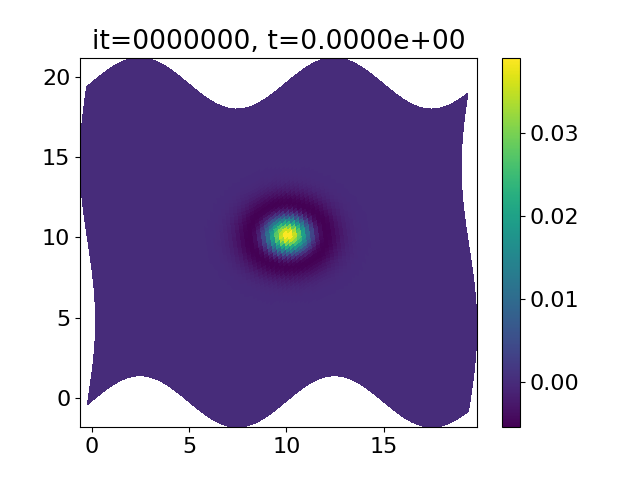
\includegraphics[width=0.475\textwidth]{Figures/vgwavy_vort_0000000.png}
  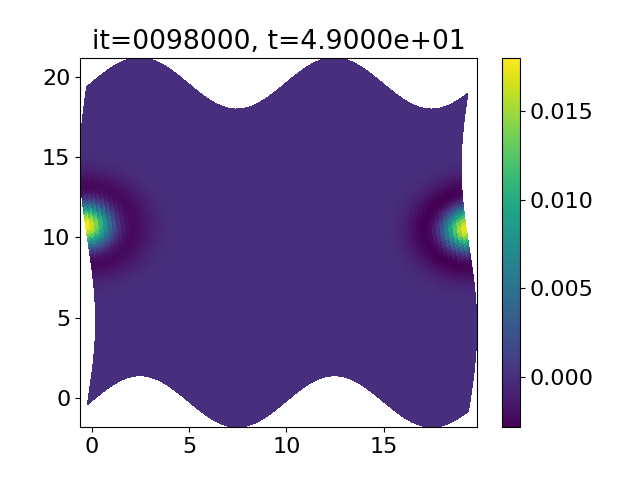
\includegraphics[width=0.475\textwidth]{Figures/vgwavy_vort_0098000.png}
  \caption{Vorticity for a periodic convecting vortex on a VGwavy grid. Left: initial condition, right: solution after 2.5 cycles.}
  \label{fig:vgwavy_vort}
\end{figure}



\clearpage

\subsection{2D Oblique Shock (\texttt{Grid.single\_ramp})}

\begin{enumerate}
\item \textbf{Computational grid:}
  \begin{itemize}
  \item $\xi_i = i\Delta\xi-L_x/2$, $i\in(0,N_\xi)$, $\Delta\xi=L_x/(N_\xi-1)$
  \item $\eta_j = j\Delta\eta$, $j\in(0,N_\eta)$, $\Delta\eta=L_y/(N_\eta-1)$
  \end{itemize}

\item \textbf{Physical-space grid:}
  \begin{itemize}
  \item Schematic shown in Fig.~\ref{fig:oblique_grid}. Ramp begins close to $x=0$ (not exactly due to ELU smoothing function).
  \item Stretching is specified as a logical argument to the grid constructor. Two options:
    \begin{enumerate}
    \item Unstretched grid.
    \item Stretched grid: reduces $\Delta x$ near $x=0$ and $\Delta y$ in boundary layers. If \texttt{BC\_eta\_top=`wall'}, then $y$-stretching is applied at the domain top and bottom. Otherwise, if \texttt{BC\_eta\_top=`farfield'}, then stretching is only applied at the domain bottom. User must supply $s_x$ and $s_y$ stretching parameters, defined below.
    \end{enumerate}
    
  \item Definition (unstretched, including ramp function $y_{R,i}$):
  \begin{align*}
    x_{ij} &= \xi_i \\
    y_{ij} &= \eta_j + y_{R,i} \\
    y_{R,i} &= (\underbrace{\alpha (\exp(\min(0,\xi_i))-1) + 1}_{\text{ELU ramp for } \xi\leq0}
    + \underbrace{\max(0,\xi_i)}_{\text{Linear ramp for } \xi>0})\tan(\delta)
    \underbrace{(1-\eta_j/L_y)}_\text{Make ramp vanish at top}
  \end{align*}
  \begin{itemize}
  \item Physical domain extents: $x\in[-L_x/2,L_x/2]$, $y\in[0,L_y]$
  \item $\alpha=1.0$
  \item $\delta$: ramp angle
  \end{itemize}
    
  \item Definition (stretched):
  \begin{align*}
    x_{ij} &= \frac{L_x}{2} \frac{\sinh(2s_x \xi_i/L_x)}{\sinh(s_x)} \\
    y_{ij} &= \frac{L_y}{2}\left(\frac{\tanh(s_y(2\eta_j/L_y - 1))}{\tanh(s_y)} + 1\right) + y_{R,i} \qquad \text{(bottom and top stretching)} \\
    y_{ij} &= L_y\left(\frac{\tanh(s_y(\eta_j/L_y - 1))}{\tanh(s_y)} + 1\right) + y_{R,i} \qquad \text{(bottom stretching only)}
  \end{align*}
  \begin{itemize}
  \item Physical domain extents: $x\in[-L_x/2,L_x/2]$, $y\in[0,L_y]$
  \item $\alpha=1.0$
  \item $s_x$, $s_y$: stretching parameters
  \item Same ramp function as uniform grid
  \end{itemize}
  \end{itemize}

\item \textbf{Grid transform:} $x_\xi,x_\eta,y_\xi,y_\eta$ are computed numerically using \texttt{Grid.grid\_transform\_2CD()}.

\item \textbf{Initial conditions:} generated from oblique-shock relations when $M_\infty>1$ and the shock is attached for the specified ramp angle $\delta$. The shock is thickened using a small hyperbolic tangent function. If the flow is subsonic or the shock is detached, then uniform flow is initialized at the freestream conditions.

\item Example solutions are shown in Fig.~\ref{fig:oblique_rho}.
  
\end{enumerate}


\begin{figure}
  \centering
  \includegraphics[width=0.75\textwidth]{Figures/oblique_grid.pdf} 
  \caption{Oblique-shock grid for $N_\xi=N_\eta=193$ and stretching factors $s_x=s_y=1.5$. Grid stretching a hyperbolic sine function in $x$ and a hyperbolic tangent function in $y$. The grid can also be refined at the top for a no-slip wall condition. (Zoom in for full resolution.)}
  \label{fig:oblique_grid}
\end{figure}

\begin{figure}
  \centering
  \includegraphics[width=0.475\textwidth]{Figures/oblique_rho_0000000.png}
  \includegraphics[width=0.475\textwidth]{Figures/oblique_rho_0163000.png}
  \caption{Density for a $M_\infty=2.1$ oblique shock through flow turning angle $\delta=15^\circ$. Left: initial condition, right: solution after 8.15 nondimensional time units. The effect of the absorbing boundary condition is evident for $x\geq 20$.}
  \label{fig:oblique_rho}
\end{figure}




\clearpage
\subsection{2D Cylinder}

The physical-space grid for the 2D cylinder case is
\begin{align*}
  x(\xi,\eta) &= R(\eta)\cos(\xi) \\
  y(\xi,\eta) &= R(\eta)\sin(\xi),
\end{align*}
where the uniform computational grid is
\begin{align*}
  \xi_i &= d\xi i, & d\xi &= 2\pi/N_\xi, & i&=0,\dotsc,N_\xi-1, \\
  \eta_j &= d\eta j, & d\eta &=1/(N_\eta-1), & j&=0,\dotsc,N_\eta.
\end{align*}
The radial grid is nonuniform using a hyperbolic-tangent stretching
\begin{equation*}
  R(\eta) = h\frac{\tanh(s_R(\eta-1))}{\tanh(s_R)} + R_\mathrm{min} + h,
\end{equation*}
where $h=R_\mathrm{max}-R_\mathrm{min}$, $R_\mathrm{min}$ is the cylinder radius, $R_\mathrm{max}$ is the radius from the center to the grid boundary, and $s_R$ is the stretching parameter.

The resulting curvilinear metrics are
\begin{align*}
  x_\xi &= -R(\eta)\sin(\xi) \\
  y_\xi &= R(\eta)\cos(\xi) \\
  x_\eta &= hs_R\, \mathrm{coth}(s_R)\,\mathrm{sech}^2(s_R(\eta-1)) \cos(\xi) \\
  y_\eta &= hs_R\, \mathrm{coth}(s_R)\,\mathrm{sech}^2(s_R(\eta-1)) \sin(\xi),
\end{align*}
where $\mathrm{coth}(z)\equiv(e^{2z}+1)/(e^{2z}-1)$ is the hyperbolic cotangent and $\mathrm{sech}(z)\equiv2/(e^z+e^{-z})$ is the hyperbolic secant.


Initial settings for the 2D cylinder grid are $N_\xi=192$, $N_\eta=128$, $R_\mathrm{min}=0.5$, $R_\mathrm{max}=25$, and $s_R=2.25$.

Todo: cylinder initial conditions.



\clearpage
\section{Code Verification} \label{sec:verification}

TBD. Finite-difference convergence: uniform \& VGwavy. Effect of artificial diffusivity: subsonic vortex convection (uniform \& VGwavy). Turbulence (boundary layer?). Adjoint convergence.



\bibliographystyle{my-elsarticle-num}
\bibliography{library.bib}



\end{document}

